%\begin{figure}[t]
%	\centering
%	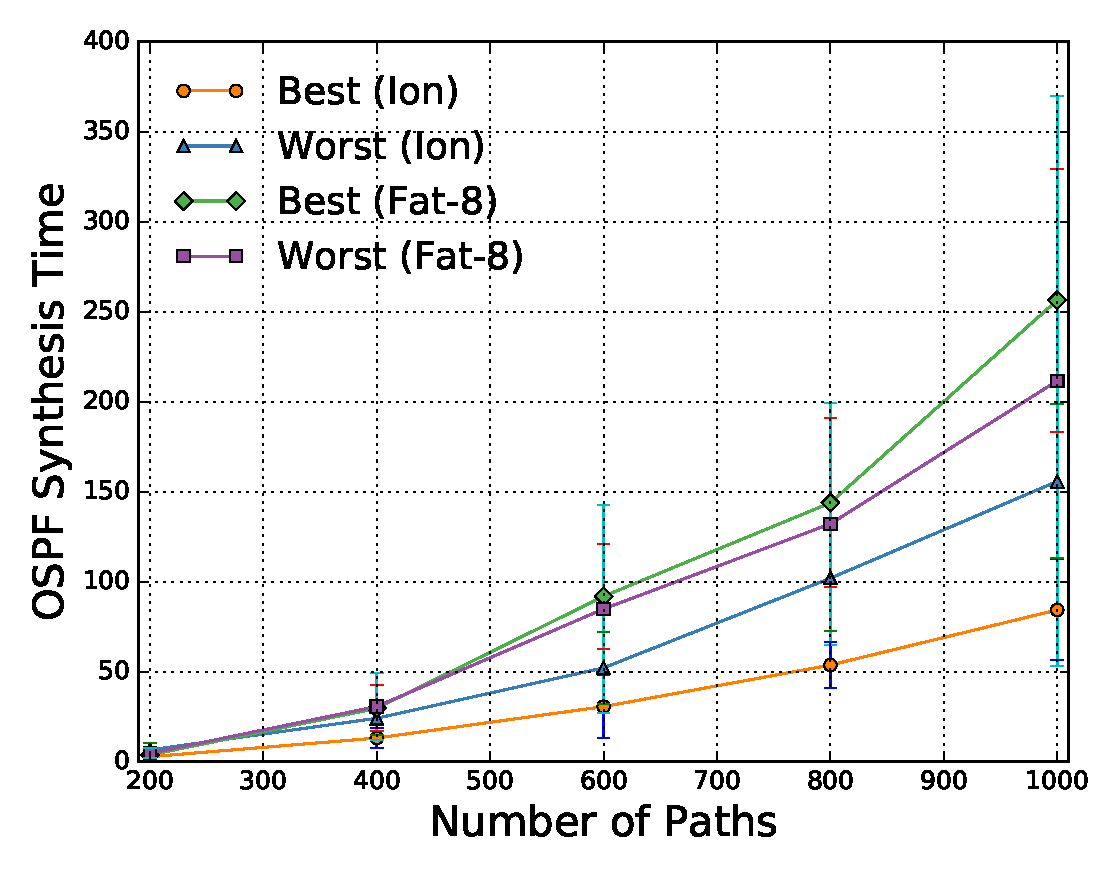
\includegraphics[width=0.7\columnwidth]{figures/ospfSynthesisTimeMCMC.eps}
%	\compactcaption{MCMC OSPF Synthesis time}
%	\label{fig:ospfmcmc}
%\end{figure}
\begin{figure*}
	\centering
	\subfloat[Synthesis Time]
	{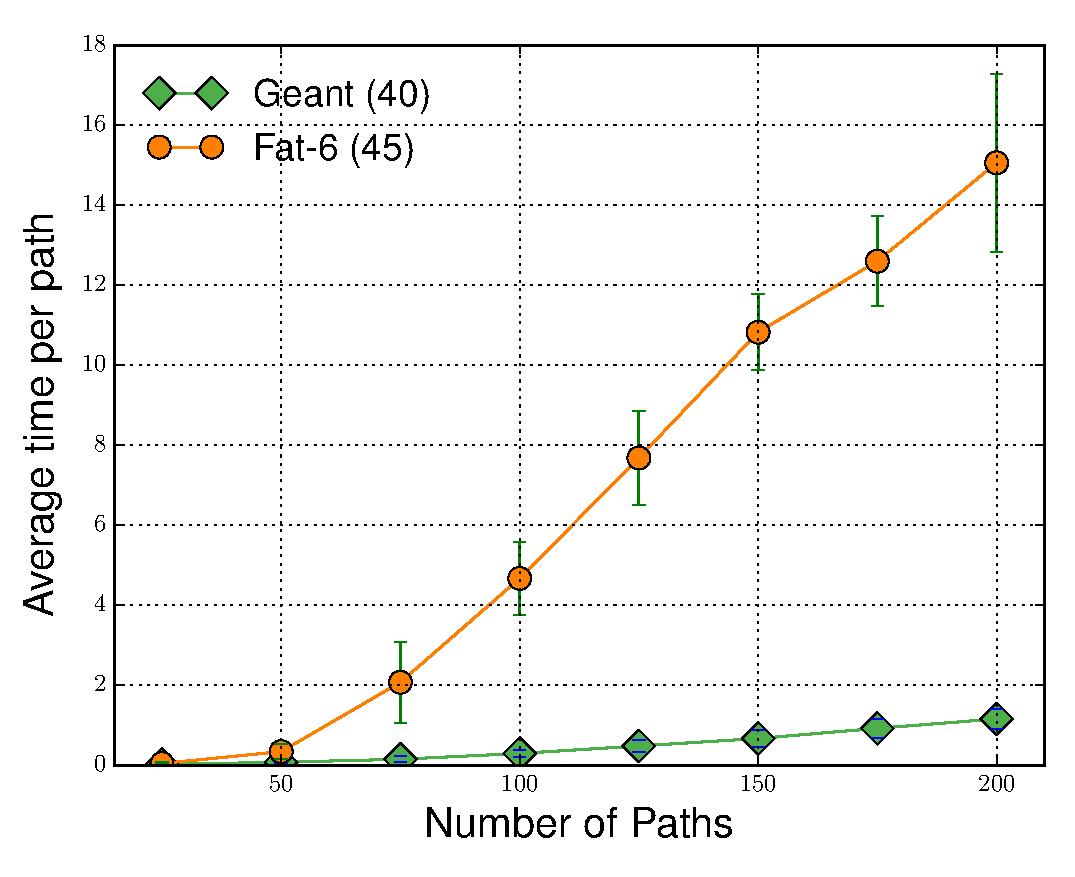
\includegraphics[width=0.66\columnwidth]{figures/ospfTime.eps}}
	\subfloat[Number of Route Filters]
	{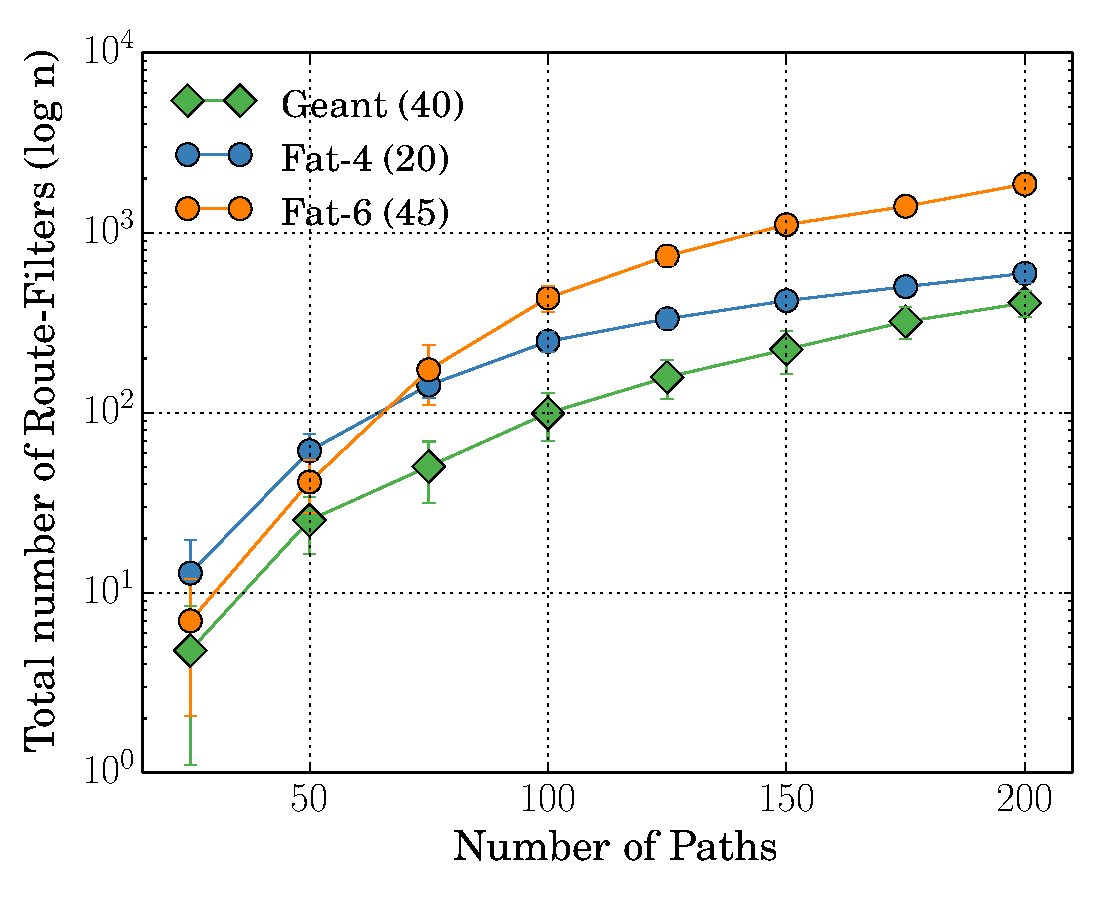
\includegraphics[width=0.66\columnwidth]{figures/ospfRF.eps}}
	\subfloat[Endpoint Resilience]
	{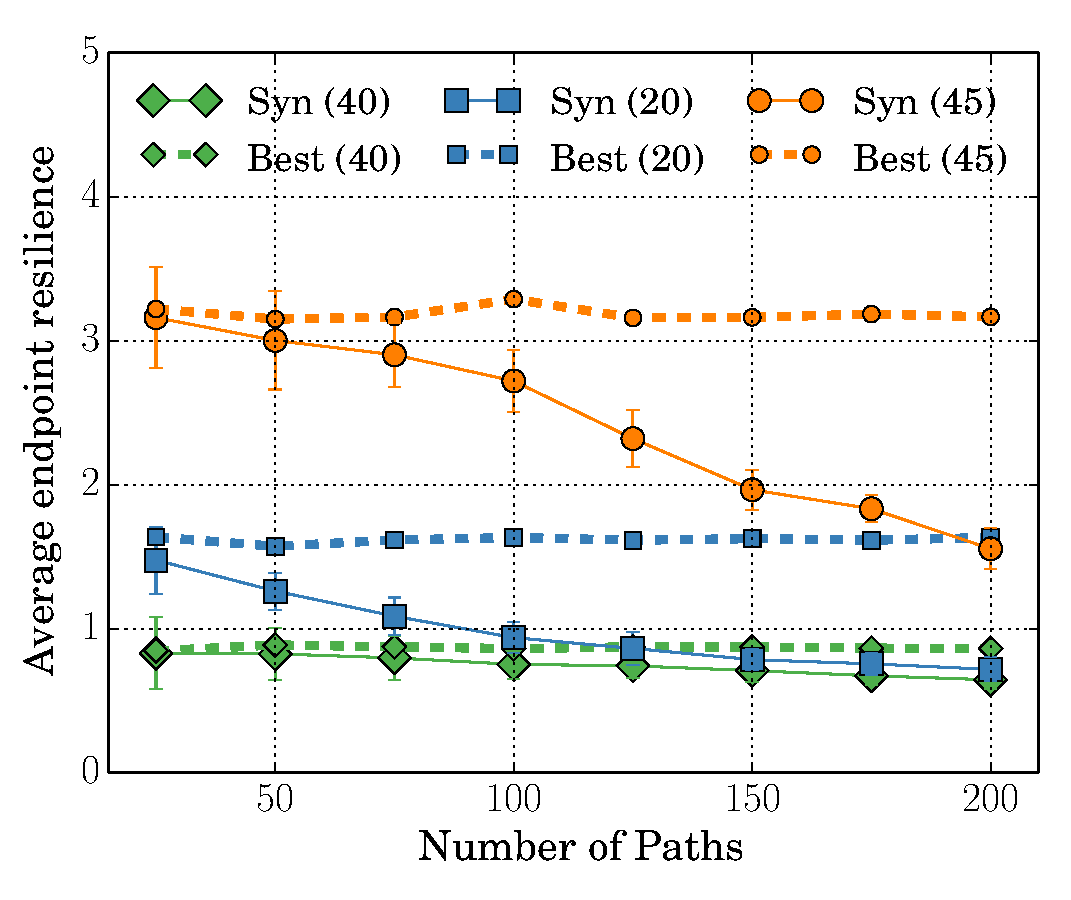
\includegraphics[width=0.66\columnwidth]{figures/ospfAvgRes.eps}}
	\compactcaption{\label{fig:ospfeval}
		OSPF Synthesis evaluation}
\end{figure*}


\begin{figure}
	\centering
	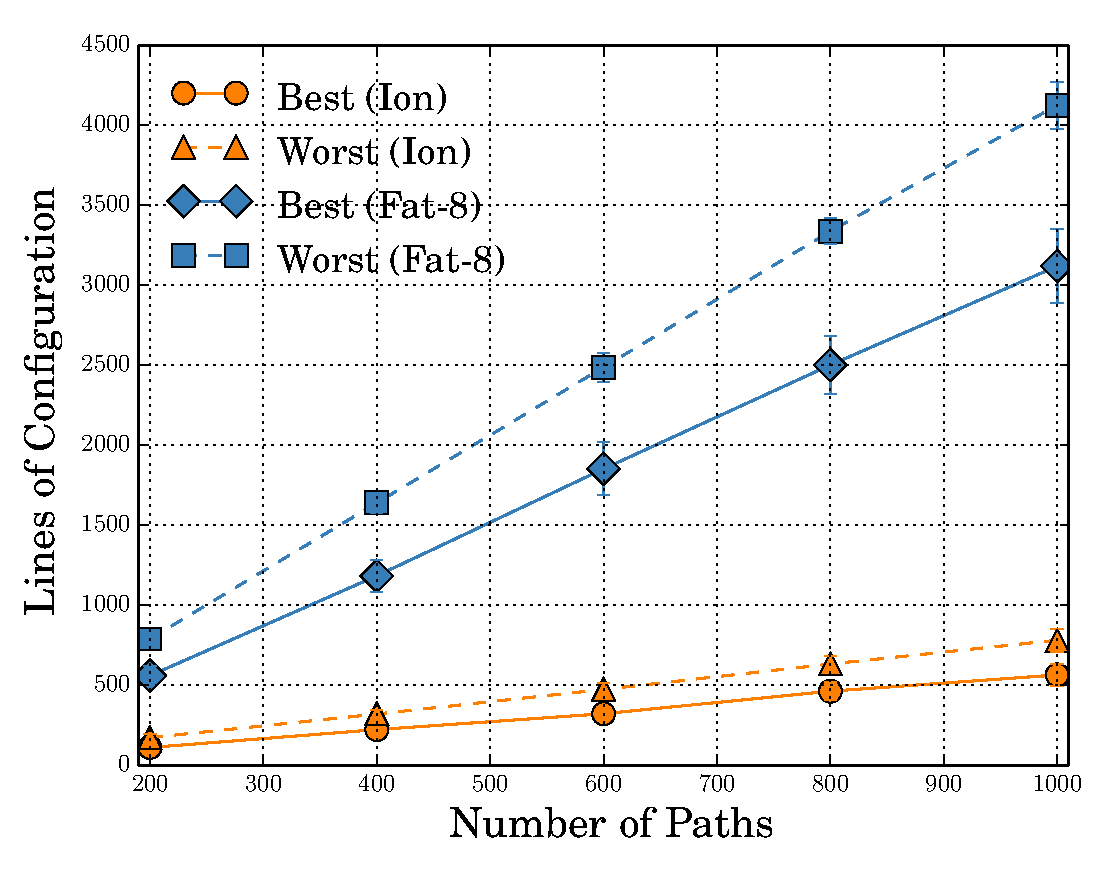
\includegraphics[width=0.7\columnwidth]{figures/confMCMC.eps}
	\compactcaption{MCMC Lines of Conf}
	\label{fig:confmcmc}
\end{figure}

\begin{figure}
	\centering
	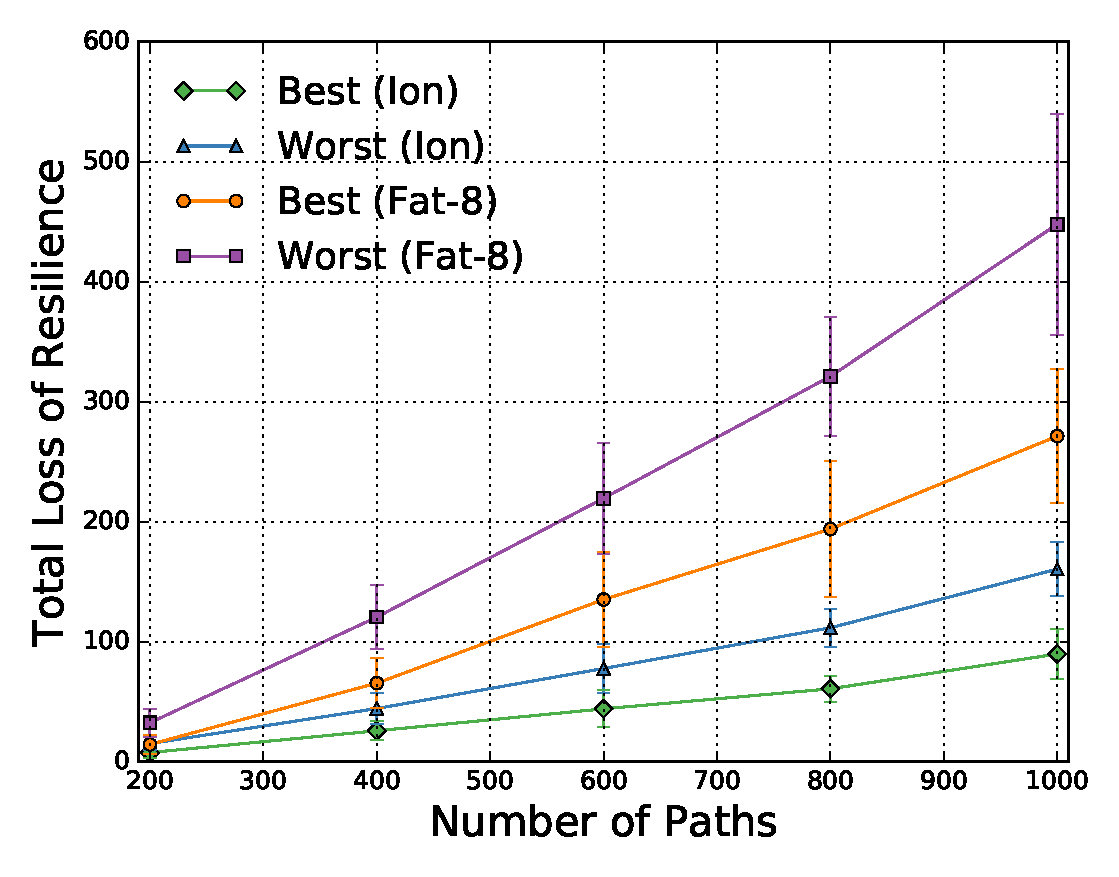
\includegraphics[width=0.7\columnwidth]{figures/TRLMCMC.eps}
	\compactcaption{MCMC TRL}
	\label{fig:trlmcmc}
\end{figure}

\begin{figure}
	\centering
	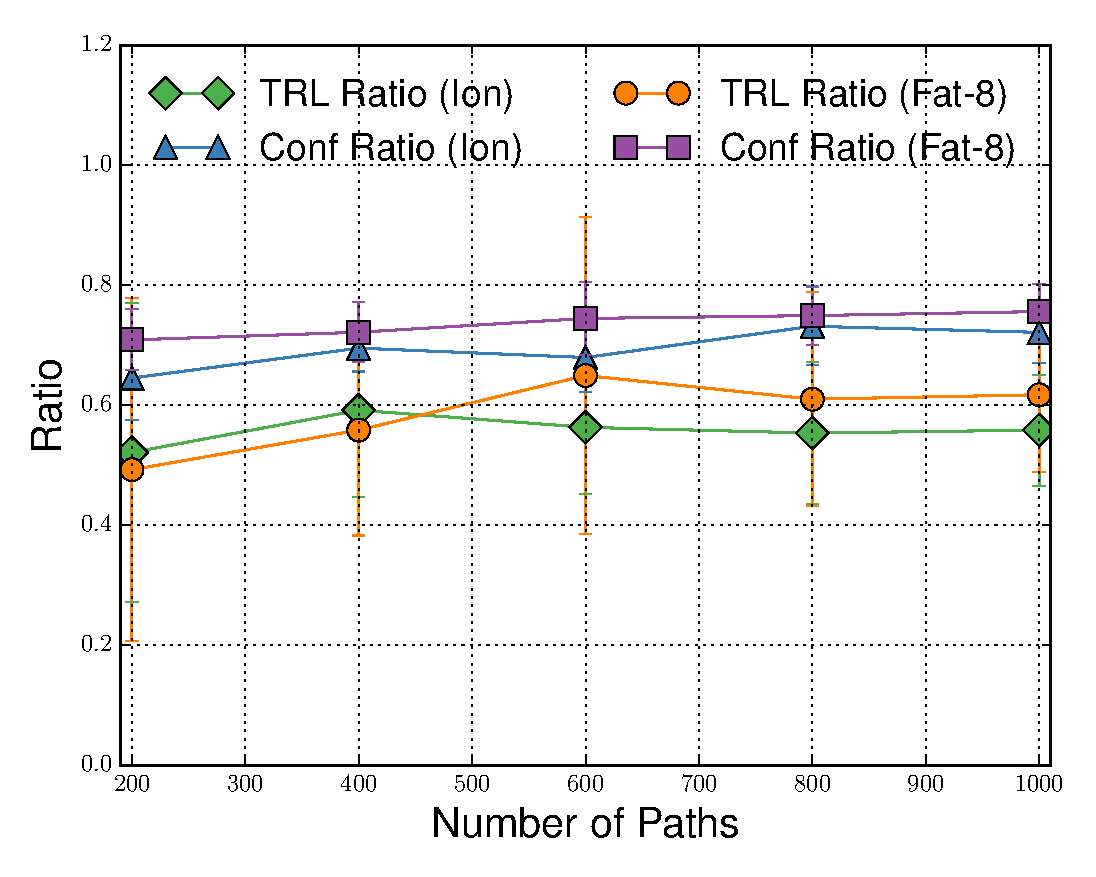
\includegraphics[width=0.7\columnwidth]{figures/ratioMCMC.eps}
	\compactcaption{MCMC Ratios}
	\label{fig:ratiomcmc}
\end{figure}




\section{Evaluation}
Ion (125 nodes) and Geant(40)

